\documentclass[10pt,letterpaper]{article}
\usepackage{graphicx}

\title{Appendix A - figures}
\date{\vspace{-5ex}}
\begin{document}
\maketitle

\begin{figure}[ht!]
	\centering
	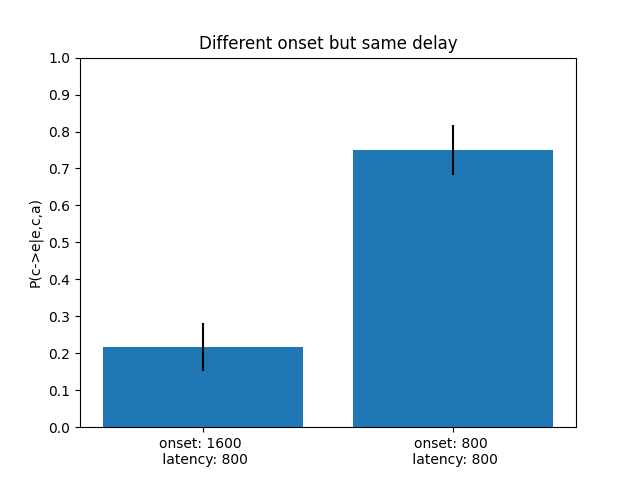
\includegraphics[width=0.8\textwidth]
	{../results/Different onset but same delay.png}
	\caption{Figure for Table 1} 
	\label{sample-figure}
\end{figure}
\begin{figure}[ht!]
	\centering
	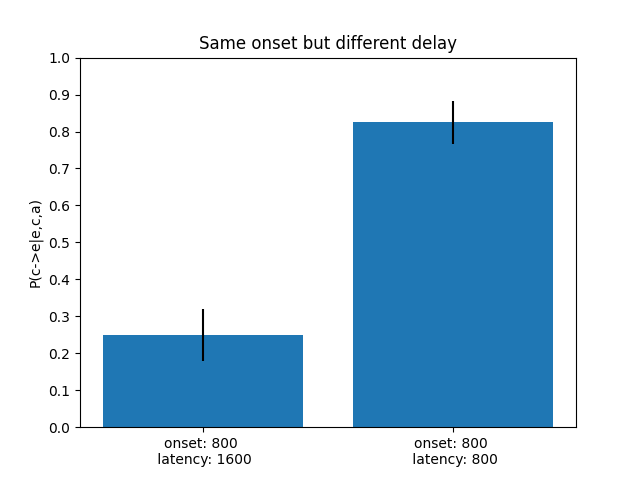
\includegraphics[width=0.8\textwidth]
	{../results/Same onset but different delay.png
	}
	\caption{Figure for Table 2} 
	\label{sample-figure}
\end{figure}
\begin{figure}[ht!]
	\centering
	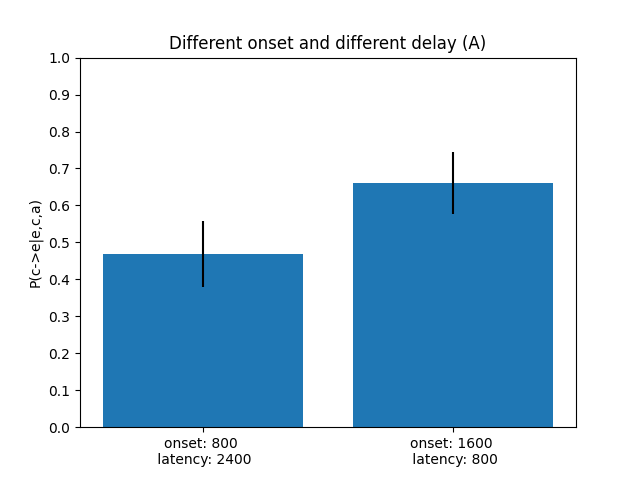
\includegraphics[width=0.8\textwidth]
	{../results/Different onset and different delay (A).png
	}
	\caption{Figure for Table 3} 
	\label{sample-figure}
\end{figure}
\begin{figure}[ht!]
	\centering
	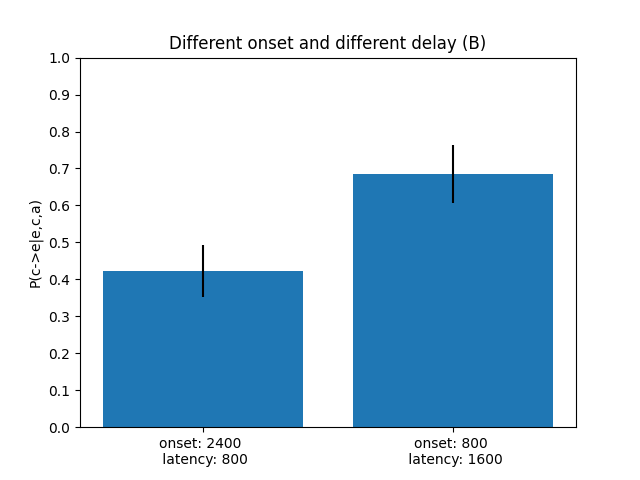
\includegraphics[width=0.8\textwidth]
	{../results/Different onset and different delay (B).png
	}
	\caption{Figure for Table 4} 
	\label{sample-figure}
\end{figure}
\begin{figure}[ht!]
	\centering
	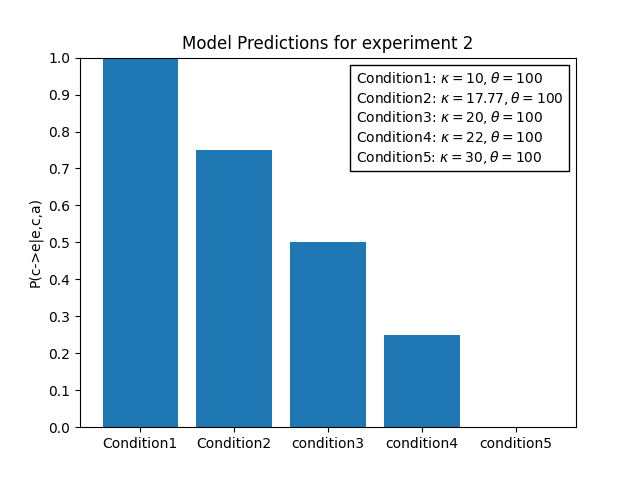
\includegraphics[width=0.8\textwidth]
	{../results/Model Predictions for experiment 2.png
	}
	\caption{Figure for Table 5} 
	\label{sample-figure}
\end{figure}
\begin{figure}[ht!]
	\centering
	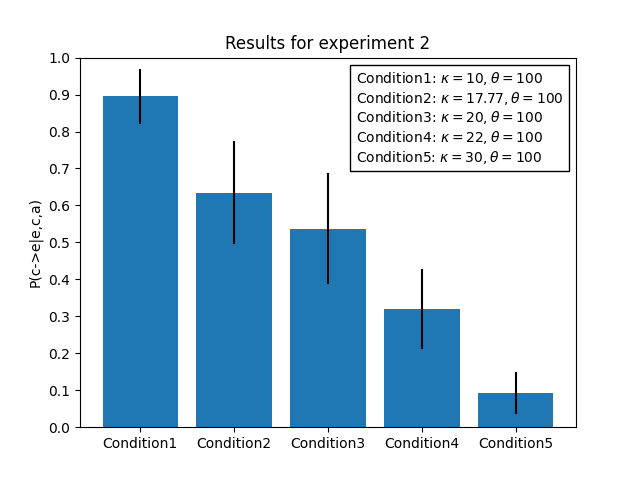
\includegraphics[width=0.8\textwidth]
	{../results/Results for experiment 2.png
	}
	\caption{Figure for Table 6} 
	\label{sample-figure}
\end{figure}
\begin{figure}[ht!]
	\centering
	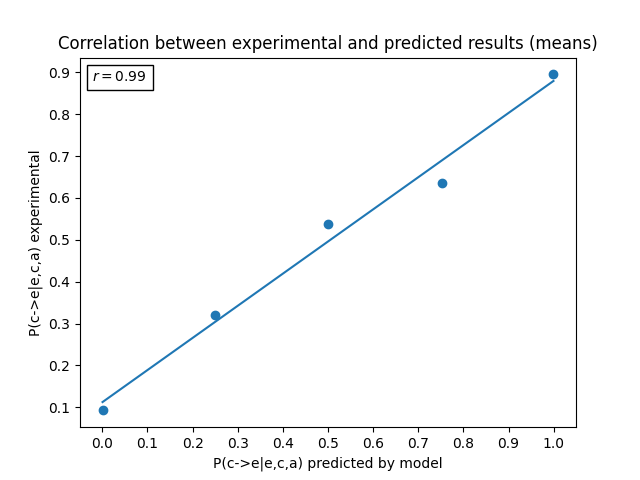
\includegraphics[width=0.8\textwidth]
	{../results/Correlation between experimental and predicted results (means).png
	}
	\caption{Figure for Experiment 2 Correlation} 
	\label{sample-figure}
\end{figure}
\begin{figure}[ht!]
	\centering
	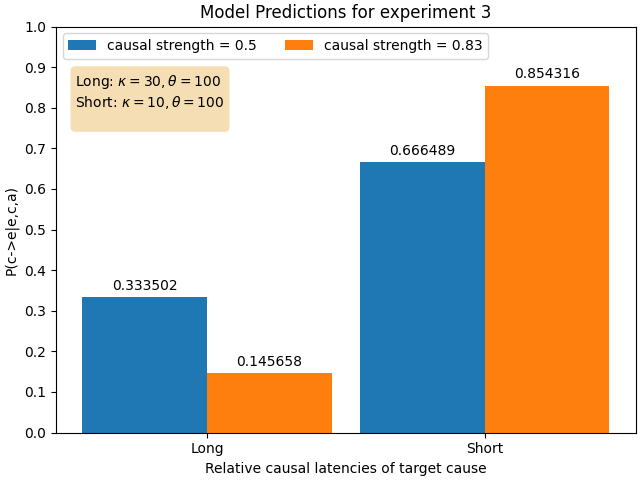
\includegraphics[width=0.8\textwidth]
	{../results/Model Predictions for experiment 3.png
	}
	\caption{Figure for table 7} 
	\label{sample-figure}
\end{figure}
\begin{figure}[ht!]
	\centering
	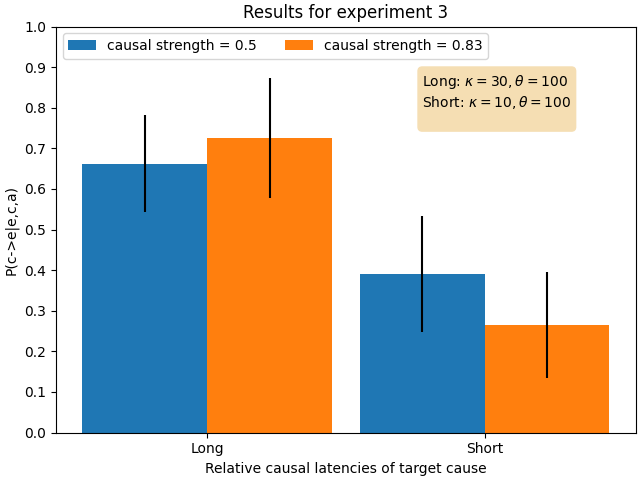
\includegraphics[width=0.8\textwidth]
	{../results/Results for experiment 3.png
	}
	\caption{Figure for table 8} 
	\label{sample-figure}
\end{figure}
\end{document}
